\cleardoublepage

\chapter{Estado de la cuestión}
\label{makereference2}

Contextualizando el entorno, la transición hacia un sistema energético descarbonizado, impulsada por la creciente penetración de fuentes de energía renovable, como la solar fotovoltaica y la eólica, presenta desafíos significativos para la estabilidad y gestión de la red eléctrica~\cite{carrasco2023battery}. De esta forma, los \gls{bess} emergen como una tecnología clave para dotar de flexibilidad al sistema, solucionando el desacoplo entre la generación y el consumo de electricidad~\cite{gissey2018market}.

El mercado eléctrico, que opera usando un modelo marginalista para los mercados spot, en donde el precio es determinado mediante el cruce de la oferta y demanda, mostrado en la figura~\ref{fig:precio-casacion} extraída directamente de extraída de \gls{omie}, ofrece diversas oportunidades para los \glspl{bess}. Estas incluyen el arbitraje de energía en los mercados spot diario, intradiarios y continuo (de mayor a menor liquidez), en los que se centra el sistema desarrollado, y la participación en los servicios de ajuste~\cite{gaspar2021optimisation}, \gls{afrr} y \gls{mfrr}, donde se ofertan disponibilidades. Por ello, la viabilidad económica depende intrínsecamente de la capacidad del sistema para formular y ejecutar estrategias de operación óptimas en un entorno de alta incertidumbre de precios y previsiones de generación~\cite{heredia2015economic}, siendo considerada incluso una ``tecnología clave para la transición energética''.

\begin{figure}
  \centering
  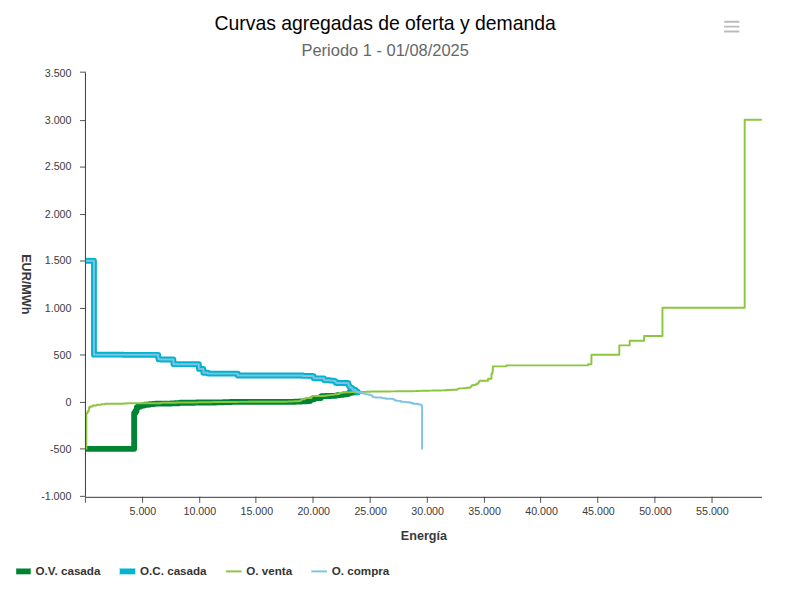
\includegraphics[width=0.75\linewidth]{figures/precio-casacion.png}
  \caption{Curva de casación real del inicio del mes de agosto del mercado eléctrico marginalista, donde tan solo las ofertas de compra por encima y de venta por debajo del precio de casación son aceptadas.}
  \label{fig:precio-casacion}
\end{figure}

\section{Situación tecnológica}
\label{makereference2.1}

Los \glspl{bess} en los mercados eléctricos, aunque prometedores, se encuentran todavía en una fase temprana de desarrollo y adopción. Esta infancia se manifiesta en la rápida evolución de los algoritmos de optimización y en la muy notable reducción de costes de la tecnología, que son características típicas de una tecnología en las primeras etapas. Dicho fenómeno se conoce como el \textit{rate of learning} e indica que ``el coste de una tecnología disminuye a medida que aumenta su producción acumulada''~\cite{mathew2021climate, louwen2018technological}, representado en la figura~\ref{fig:rate-of-learning}.

\begin{figure}
  \centering
  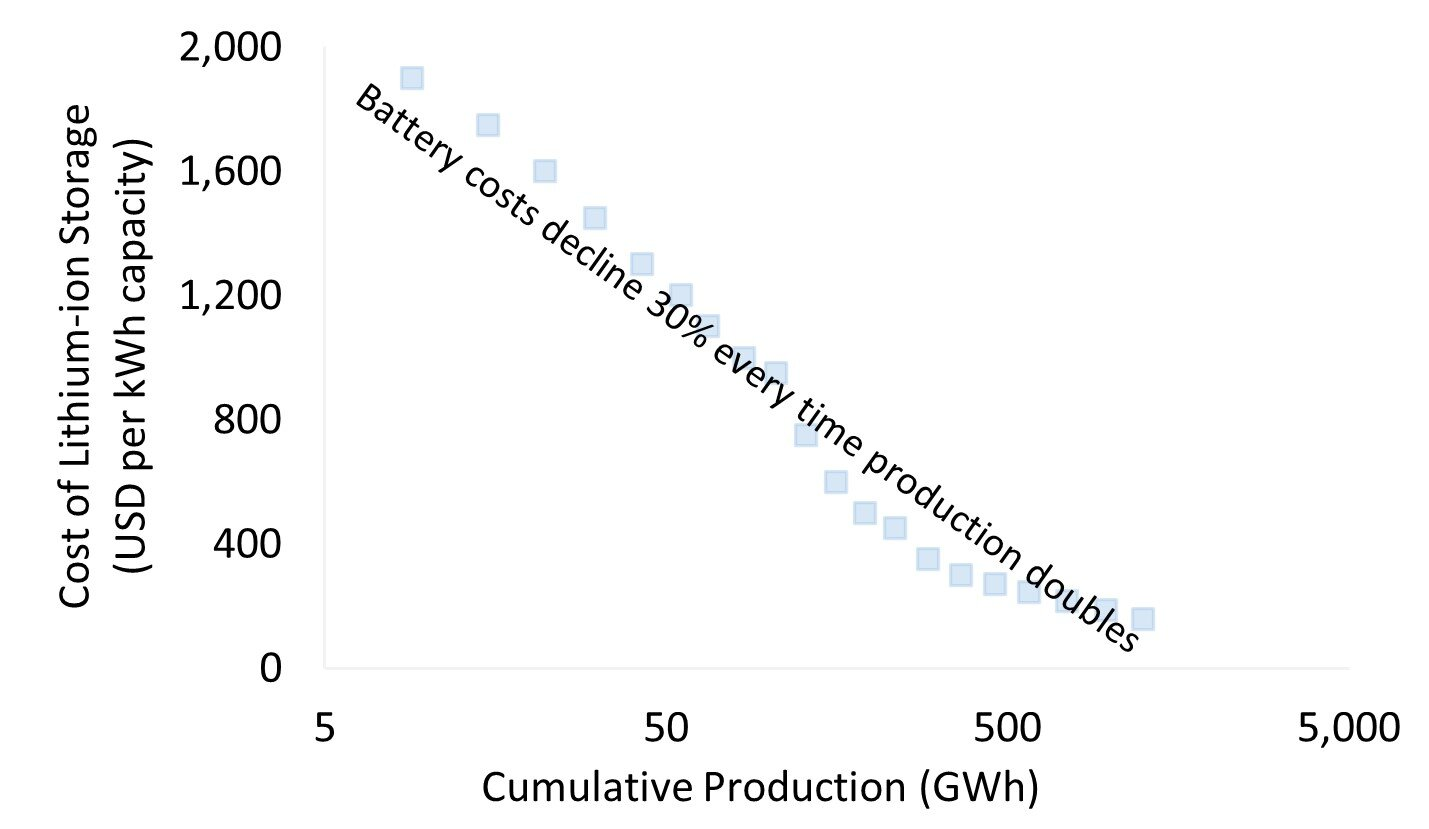
\includegraphics[width=0.75\linewidth]{figures/rate-of-learning.jpg}
  \caption{Representación de la reducción de los costes de las baterías según su uso, se observa una reducción del 10--35\% cada vez que se dobla la producción~\cite{irena2025irena}.}
  \label{fig:rate-of-learning}
\end{figure}

Por ello, la situación tecnológica de los optimizadores de \glspl{bess} varía significativamente entre el mercado eléctrico ibérico, europeo y demás, debido a diferencias en el diseño, marcos regulatorios e incentivos políticos.

Por un lado, el mercado ibérico, el pertinente al desarrollo realizado, presenta tanto oportunidades como barreras para los \glspl{bess}, y es que el altamente notorio apoyo de las tecnologías renovables crea una volatilidad de precios\footnote{Debido a la cantidad de activos solares, por ejemplo, los precios se desploman cuando hace sol, pero cuando no hay recursos renovables, los precios pueden llegar a dispararse, teniendo que hacer uso de tecnologías energéticas más caras}, que puede ser aprovechada mediante el arbitraje de energía~\cite{hu2022potential}, observado en la figura~\ref{fig:arbitraje-tecnologia}. Sin embargo, la regulación española ha sido anteriormente considerada una de las principales barreras~\cite{hu2021barriers} con lo relacionado a las tasas energéticas (al cargar y descargar de la red), aunque la normativa evoluciona para mitigar estos problemas con grandes ayudas del estado dirigidas a las baterías, en este caso. En la actualidad, se subraya que la producción del mercado iberico es infima en comparación, figura~\ref{fig:comparacion-energia-ciclada} obtenida directamente de \gls{ree}, pero estudios económicos muestran la viabilidad potencial de los \gls{bess} si se implementa una estrategia de optimización adecuada~\cite{he2015optimal}.

\begin{figure}
  \centering
  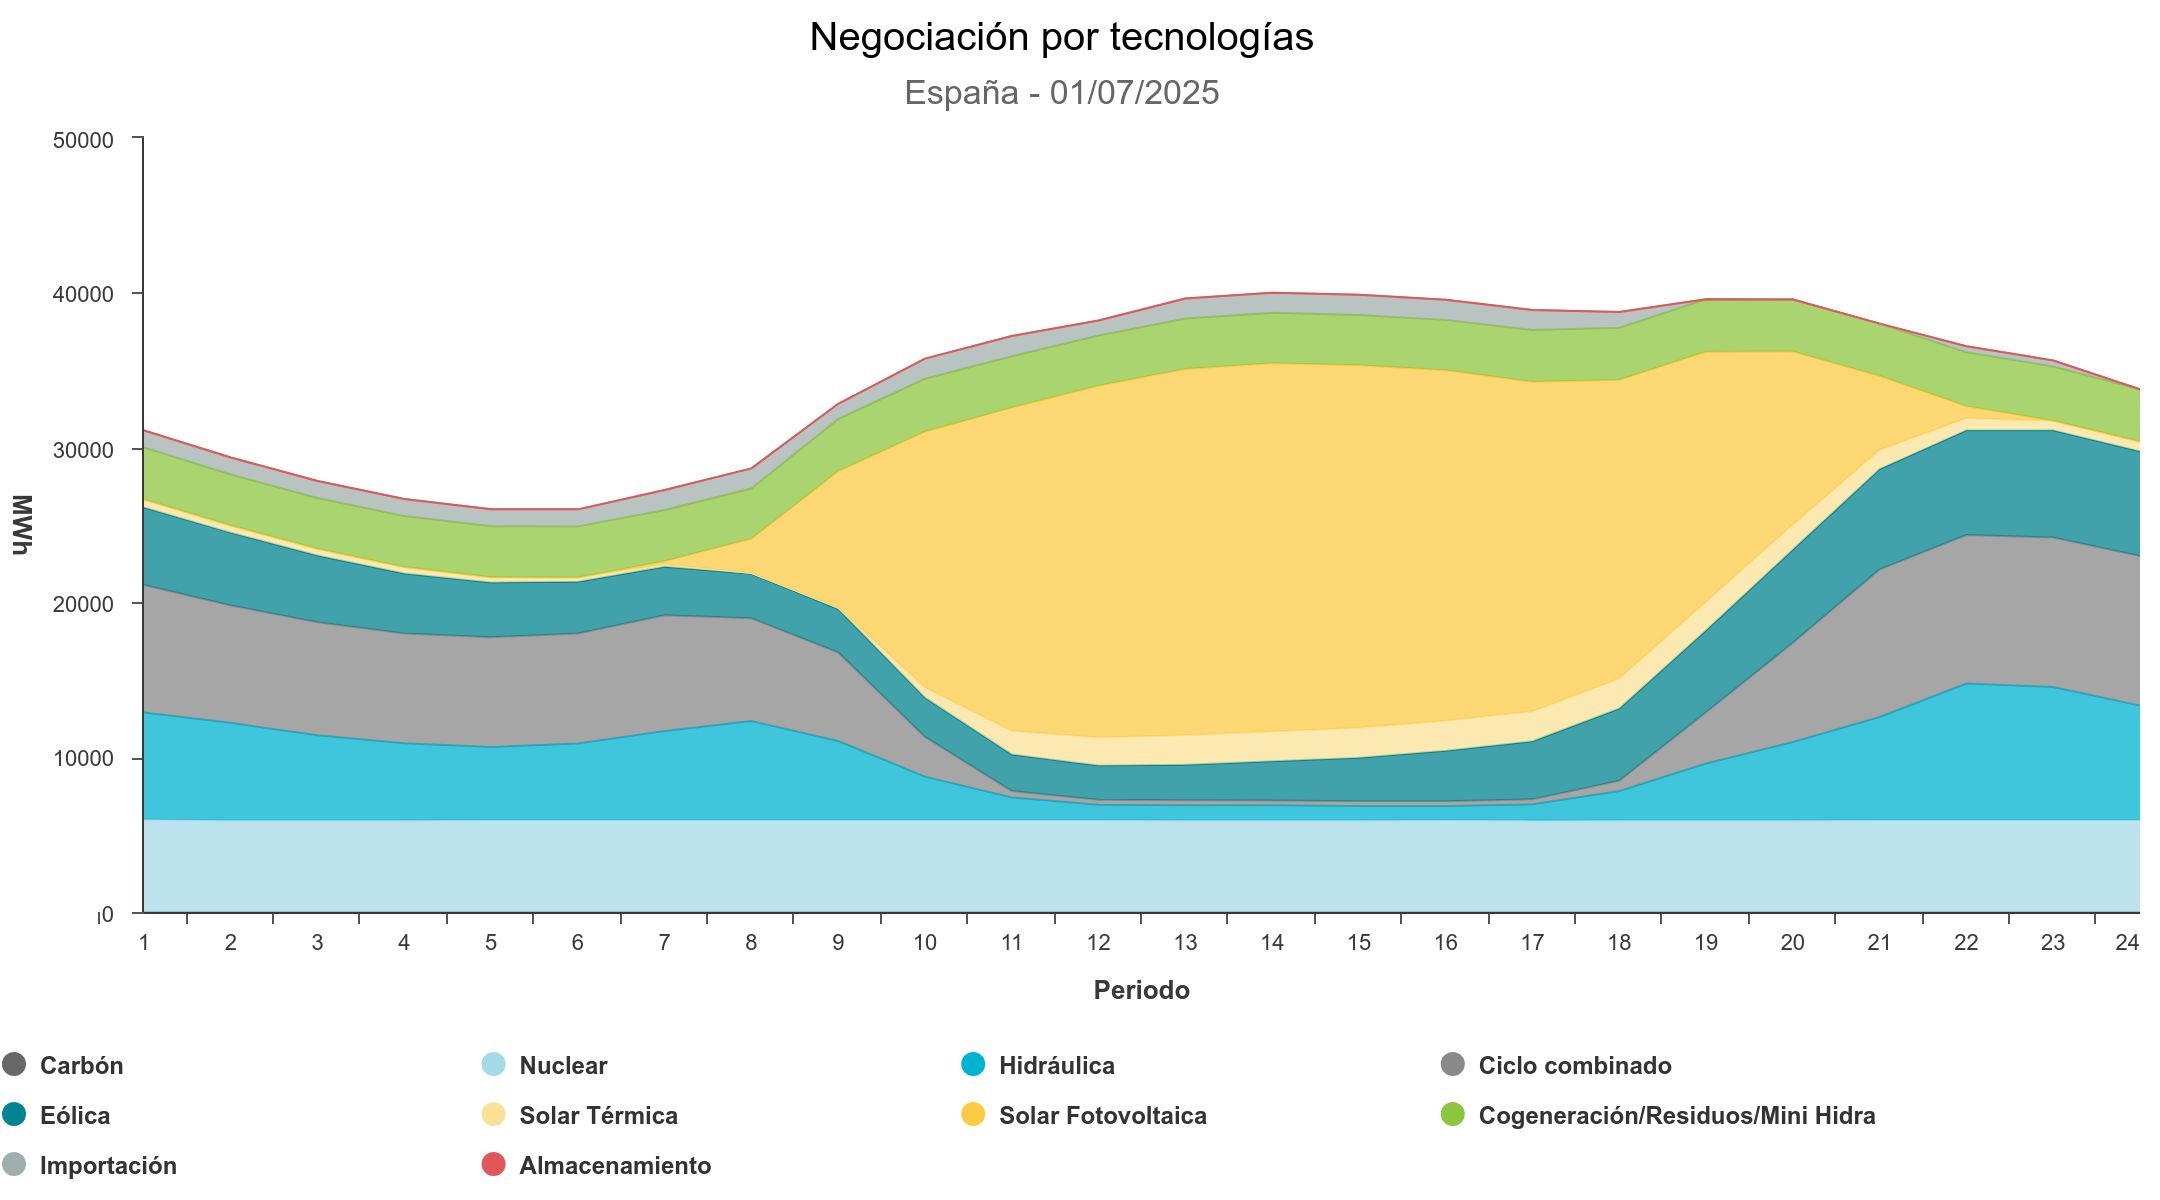
\includegraphics[width=0.75\linewidth]{figures/arbitraje-tecnologia.jpg}
  \caption{Negociación por tecnologías del inicio del mes de junio, donde las tecnologías más caras, como el ciclo combinado, abarcan la mayor parte de la generación cuando no hay tanto recurso renovable.}
  \label{fig:arbitraje-tecnologia}
\end{figure}

\begin{figure}
  \centering
  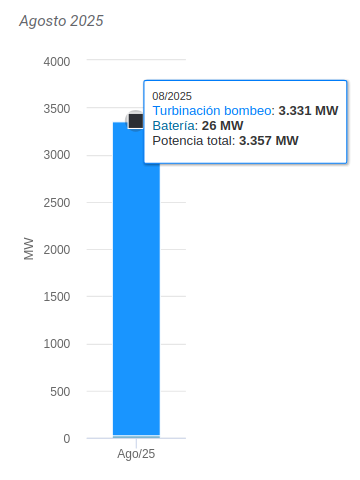
\includegraphics[width=0.5\linewidth]{figures/comparacion-energia-ciclada.png}
  \caption{Comparación entre la media de la energía diaria real arbitrada durante mes de agosto entre el bombeo y las baterías de Optibat.}
  \label{fig:comparacion-energia-ciclada}
\end{figure}

A nivel europeo, países como Alemania y Reino Unido han sido los pioneros en la integración de \glspl{bess}~\cite{kivipelto2017grid, tejada2019review}, principalmente a través de mercados de regulación de frecuencia desorbitadamente remunerados, aunque la saturación de estos mercados este llevando a una mayor dependencia de los ingresos del arbitraje de energía en los mercados spot (relacionados con el trabajo realizado). De esta forma, los mercados europeos encaminan la situación futura del mercado ibérico, como se ve reflejado en la actualidad~\cite{kumar2019strategic}.

\section{Estrategias de optimización}
\label{makereference2.2}

